\vspace{0.2in}  %to enter vertical space
\begin{enumerate}
\item{\textbf{\underline{Setting the units:}}
You can set the units for your drawing from Edit Menu.
    \begin{figure}[h!]
    \centering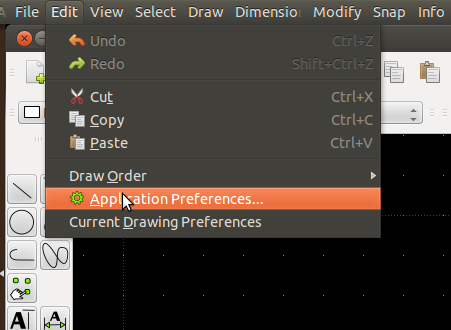
\includegraphics[width=200px]{./images/edit.png}
    \caption{\small \sl Edit menu}
    \end{figure}\\
You can either set your changes as a whole or for a current drawing.
If you make changes in \textbf{Application Preferences}, then these changes will reflect to your whole application.
And If you make changes in \textbf{Current Application Prefences}, then the changes reflect to your current Drawing only.\\\\
To set changes in your Current Drawing:
    \begin{enumerate}
    \item{Click on the \textbf{Edit} Menu}
    \item{then click on \textbf{Current Drawing Preferences}}
       \begin{figure}[h!]
       \centering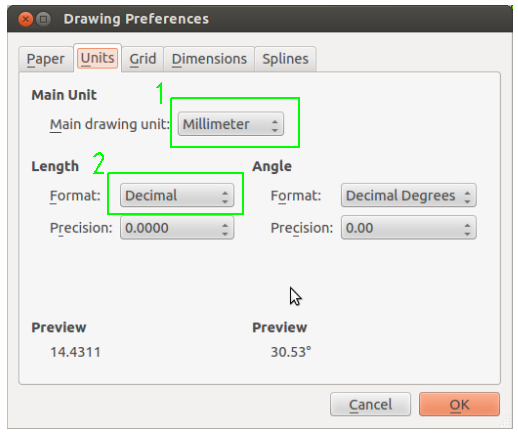
\includegraphics[width=200px]{./images/draw_pref.png}
       \caption{\small \sl Current Drawing Preference}
       \end{figure}
    \item{Goto \textbf{Units} tab,The units command allows setting the type of measurement and orientation of angular measurement.}
    \item{Select the \textbf{Main Drawing unit}. By default, it is set to Millimeter.}
    \item{Set the Format. There are different formats: Architectural, Decimal, Engineering, Fractional, Scientific.}
       \begin{figure}[h!]
       \centering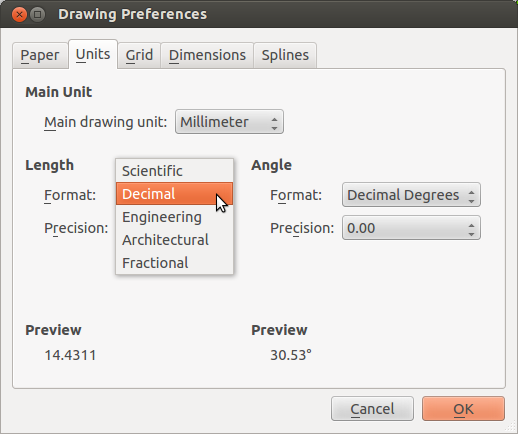
\includegraphics[width=200px]{./images/unitFormat.png}
       \caption{\small \sl Setting the Format for Length.}
       \end{figure}
    \end{enumerate}
}
\vspace{0.2in}
\item{\underline{\textbf{Snap and grid mode:}} Grid and Snap mode are used to learn, to restrict the movement of the cursor to a set increment on the screen. The GRID and SNAP MODE options can be turned ON or OFF from the icons or menubar or command line.\\
\textbf{Snap} feature allows you to precisely select grid points or significant points on existing objects: endpoints or midpoints of lines, etc. You can select snap option under 'Snap' Menu or from icons or from command line. Below is this image of icons of different type of snapping.
\vspace{.2in}
\begin{figure}[h!]
\begin{minipage}{.5\textwidth}
\centering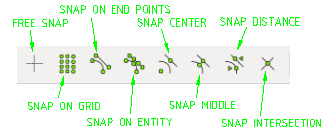
\includegraphics[width=210px]{./images/snap.png}
\caption{\small \sl Icons for Snapping}
\end{minipage}
\begin{minipage}{.5\textwidth}
       \centering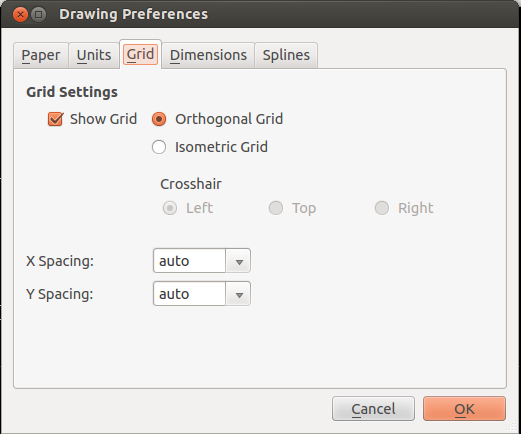
\includegraphics[width=180px]{./images/gridSet.png}
       \caption{\small \sl Choosing the type of Grid.}
       \end{minipage}
       \end{figure}}
\newpage
The \textbf{Grid\centering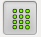
\includegraphics[width=20px]{./images/grid.png}}: A grid usually refers to two or more infinite sets of evenly-spaced parallel lines at particular angles to each other in a plane, or the intersections of such lines. It helps you align objects and visualize the distance between them. You can also change the color of Grid from Edit menu $>$ Application Prefences $>$ Grid color.\\
There are two types of grid: \textbf{orthogonal grids}, with two sets of lines perpendicular to each other (such as the square grid), and \textbf{isometric grids}, with three sets of lines at 60-degree angles to each other (such as the triangular grid). Isometric grid is used to depict 3D objects on a 2D surface.You can select type of Grid you want from Edit menu $>$ Current Drawing Preferences.
\vspace{0.2in}
\item{\textbf{\underline{\\Zooming and panning:}} Pan and zoom are very useful tools in LibreCAD. We can use Zoom or Pan command to navigate in our drawing.
\begin{figure}[h!]
\centering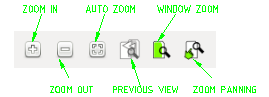
\includegraphics[width=240px]{./images/zoomPan.png}
\caption{\small \sl Icons for Zooming and Panning}
\end{figure}
\textbf{\\Zoom:} This tool increases / decreases the current viewing factor. The zoom tool is valuable when
you need to move up close to an entity to work on it. This is especially true when the
area is very small, or several lines drawn close together. As you will see in a moment,
there are several ways to use zoom: Zoom In, Zoom out, Auto Zoom, Window Zoom, Zoom panning.\\
\textbf{Panning:} Panning means moving around the drawing. Selecting the panning option you can drag your drawing. Pan allows you to dragging the drawing up, down, right, or left. This is especially useful if your drawing is large.}
\vspace{0.2in}
\item{\textbf{\underline{Dimentioning:}} To make changes in your application, goto `Application prefernces' under `Edit' menu. If you want to make changes in current drawing only, then goto to \textbf{Edit} $>$ \textbf{Current Preference}. Then selects the \textbf{Dimensions} tab.   
       \begin{figure}[h!]
       \centering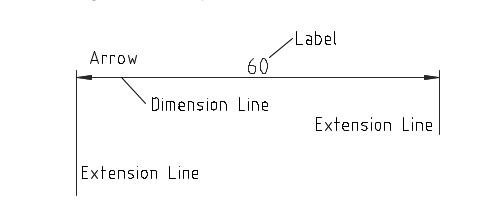
\includegraphics[width=230px]{./images/dimen.png}
       \caption{\small \sl Dimensioning}
       \end{figure}
       \begin{figure}[h!]
       \centering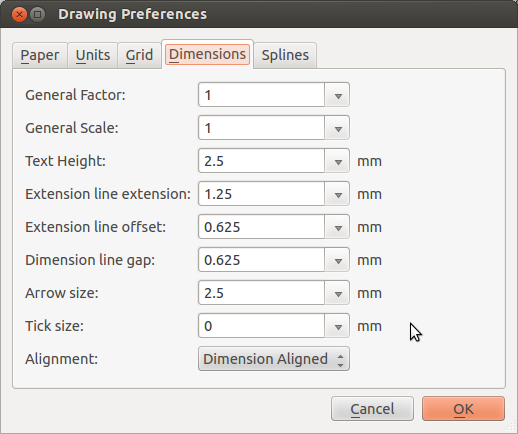
\includegraphics[width=200px]{./images/dimensions.png}
       \caption{\small \sl Setting Dimensioning for Drawing.}
       \end{figure}
}
%\vspace{0.2in}
\item{\underline{\textbf{\\\\Layers:}} Every entity of a drawing is on exactly one layer and a layer can contain
lots of entities. Typically entities with a common 'function' or common attributes are
put on the same layer. Layers are especially important in Assembly drawings. An Assembly drawing is a
drawing showing 2 or more parts as an assembly on a drawing. Each part is drawn on
its own layer and when all the layers are shown on the drawing you have the complete
assembly in view. You can create/ delete as much layers as you want, but their must be atlest one layer in drawing. By default there is one layer created, named `\textbf{0}'. Layers can have attributes (color, line width, line
style). Each entity can have its own attributes or have its attributes defined by the
layer it is placed on.
\begin{figure}[h!]
       \centering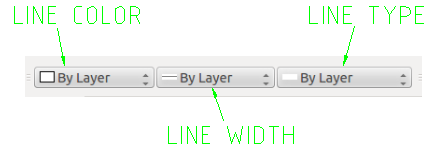
\includegraphics[width=230px]{./images/layer_set.png}
       \caption{\small \sl Icons for Layer}
       \end{figure}
     \begin{itemize}
     \item{\textbf{Line color:} You can select the color for your layer. This color will be same for all entities on a current Layer.}
     \item{\textbf{Line width:} You can select the width of line you want to use for your current layer.}
     \item{\textbf{Line type:} It provides you different types of lines: Dot, Dashed, Continous, Divid, Center, Border, No pen, etc.}
     \end{itemize}}
\end{enumerate}
